\documentclass[mathserif, handout]{beamer}
% ======================================================================
% General LaTeX Setup for Beamer (Reusable Preamble)
% Author: Chandra Gummaluru
% ======================================================================

\documentclass[mathserif, handout]{beamer}
\setbeamertemplate{frametitle}{}

% ------------------------------------------------------------
% basic packages
% ------------------------------------------------------------
\usepackage{url}
\usepackage{ifthen}
\usepackage{enumerate}
\usepackage[font=small]{caption}
\usepackage{subcaption}
\usepackage{moresize}
\usepackage[outline]{contour}
\usepackage{transparent}
\usepackage{worldflags}
\usepackage{bm}
\usepackage{graphbox}
\usepackage{mathtools}
\usepackage{multirow}
\usepackage{fontawesome5}
\usepackage{pifont}
\usepackage{array}
\usepackage{comment}

% ------------------------------------------------------------
% math
% ------------------------------------------------------------
\DeclarePairedDelimiter{\floor}{\lfloor}{\rfloor}
\DeclarePairedDelimiter{\ceil}{\lceil}{\rceil}

% ------------------------------------------------------------
% colors
% ------------------------------------------------------------
\definecolor{hl}{RGB}{248,196,69}
\definecolor{myred}{HTML}{ED5565}
\definecolor{myorange}{HTML}{FC6E51}
\definecolor{myyellow}{HTML}{FFCE54}
\definecolor{mycyan}{HTML}{4FC1E9}
\definecolor{myblue}{HTML}{5D9CEC}

\newcommand{\graytext}[1]{\footnotesize\color{gray}#1\normalsize\color{black}}

% ------------------------------------------------------------
% symbols
% ------------------------------------------------------------
\newcommand{\cmark}{\ding{51}}
\newcommand{\xmark}{\ding{55}}

% ------------------------------------------------------------
% highlighting
% ------------------------------------------------------------
\newcommand{\reducedstrut}{\vrule width 0pt height .9\ht\strutbox depth .9\dp\strutbox\relax}
\newcommand{\highlight}[1]{%
  \begingroup\setlength{\fboxsep}{0pt}\colorbox{hl}{\reducedstrut$\displaystyle #1$\/}\endgroup}
\newcommand{\highlightc}[2]{%
  \begingroup\setlength{\fboxsep}{0pt}\colorbox{#1}{\reducedstrut$\displaystyle #2$\/}\endgroup}

% ------------------------------------------------------------
% environments (boxes)
% ------------------------------------------------------------
\usepackage{tcolorbox}
\tcbuselibrary{skins}

\newtcolorbox{thmbox}[1][]{colback=gray!30!white!20, colframe=black, fonttitle=\bfseries, title=#1, boxrule=0.5pt}

% 1) Bottom open (draw top + sides only)
\newtcolorbox{thmboxtop}[1][]{
    enhanced,
    frame hidden,
    colback=gray!30!white!20,
    borderline north={0.5pt}{0pt}{black}, % top
    borderline west={0.5pt}{0pt}{black},  % left
    borderline east={0.5pt}{0pt}{black}   % right
}

% 2) Top open (draw bottom + sides only)
\newtcolorbox{thmboxbot}[1][]{
    enhanced,
    frame hidden,
    colback=gray!30!white!20,
    borderline south={0.5pt}{0pt}{black}, % bottom
    borderline west={0.5pt}{0pt}{black},  % left
    borderline east={0.5pt}{0pt}{black}   % right
}

% 3) Side only (draw only left and right)
\newtcolorbox{thmboxside}[1][]{
    enhanced,
    frame hidden,
    colback=gray!30!white!20,
    borderline west={0.5pt}{0pt}{black},  % left
    borderline east={0.5pt}{0pt}{black}   % right
}

\newtcolorbox{defboxtop}[1][]{
    enhanced,
    colback=gray!30!white!20,
    frame hidden,
    overlay={
        % Draw top + sides with rounded corners
        \draw[line width=0.5pt, black, rounded corners=3mm]
            (frame.south west) -- (frame.north west) -- (frame.north east) -- (frame.south east);
    },
    #1
}

\newtcolorbox{defboxbot}[1][]{
    enhanced,
    colback=gray!30!white!20,
    frame hidden,
    overlay={
        % Draw top + sides with rounded corners
        \draw[line width=0.5pt, black, rounded corners=3mm]
            (frame.north west) -- (frame.south west) -- (frame.south east) -- (frame.north east);
    },
    #1
}

\newtcolorbox{defboxside}[1][]{
    enhanced,
    frame hidden,
    colback=gray!30!white!20,
    borderline west={0.5pt}{0pt}{black},  % left
    borderline east={0.5pt}{0pt}{black}   % right
}

\newtcolorbox{proofbox}[1][]{colback=gray!20!white!20, colframe=grey, fonttitle=\bfseries, title=#1, boxrule=0.5pt, colbacktitle=white, enhanced jigsaw, sharp corners}

% ------------------------------------------------------------
% code listings
% ------------------------------------------------------------
\usepackage{listings}
\lstdefinestyle{mypython}{
  language=Python,
  deletekeywords=[2]{open, next, from, chr, str, int},
  morekeywords=[3]{List, Graph, Tree, Dict, Set, UnionFind, Ordict, Trie, Queue},
  morekeywords=[4]{ListNode, Vertex, Edge, Path, TreeNode, DictNode, UnifNode, OrdictNode, TrieNode, QueueNode},
  morekeywords=[5]{True, False, Boolean, String, Integer, Key, Function, KeyedObject, Object, Array, Tuple, Optional, None},
  keywordstyle=\color{mycyan}\bfseries,
  keywordstyle=[3]\color{myblue}\bfseries,
keywordstyle=[4]\color{myblue}\bfseries,
keywordstyle=[5]\color{mycyan}\bfseries,
  stringstyle=\color{orange},
  commentstyle=\color{gray}\itshape,
  basicstyle=\ttfamily\footnotesize,
  numbers=left,
  numberstyle=\tiny\color{gray},
  stepnumber=1,
  numbersep=5pt,
  xleftmargin=15pt,
  frame=none,
  showstringspaces=false,
  breaklines=true,
  breakatwhitespace=true,
  tabsize=4,
  columns=flexible
}


% ------------------------------------------------------------
% algorithms
% ------------------------------------------------------------
\usepackage{algorithm}
\usepackage[endLComment=~]{algpseudocodex}
\makeatletter
\algrenewcommand\ALG@beginalgorithmic{\footnotesize}
\makeatother

% ------------------------------------------------------------
% optimization environments
% ------------------------------------------------------------
\usepackage[nocomma]{optidef}

% ------------------------------------------------------------
% pgfplots and pie charts
% ------------------------------------------------------------
\usepackage{pgfplots}
\usepackage{pgf-pie}
\pgfplotsset{compat=1.7}

% ------------------------------------------------------------
% tikz
% ------------------------------------------------------------
\usepackage{tikz}
\usetikzlibrary{
  angles, quotes, positioning, fit, backgrounds, shapes.geometric, intersections,
  calc, shapes, mindmap, decorations.text, arrows, arrows.meta,
  automata, chains, decorations.pathreplacing, calligraphy,
  decorations.markings, shapes.misc, decorations.pathmorphing
}
\tikzset{
  invisible/.style={opacity=0},
  visible on/.style={alt=#1{}{invisible}},
  alt/.code args={<#1>#2#3}{\alt<#1>{\pgfprioritysalso{#2}}{\pgfprioritysalso{#3}}}
}

\newcommand{\multiedge}[5][]{
\pgfmathsetmacro{\N}{#4}
\pgfmathsetmacro{\mid}{(\N-1)/2}
\foreach \i in {0,...,\numexpr#4-1\relax} {

\pgfmathsetmacro{\k}{\i-\mid}
\draw[#1] ($ (#2) + \k*#5*($(#2)!1!90:(#3)$) $) -- ($ (#3) + \k*#5*($(#2)!1!90:(#3)$) $); 

}
\draw[#1,  -{>[scale=1]}]
  ($(#2)!0.54!(#3)$) -- ($(#2)!0.55!(#3)$);
}

% ------------------------------------------------------------
% bibliography
% ------------------------------------------------------------
\usepackage[style=ieee]{biblatex}
\setbeamertemplate{bibliography item}{\insertbiblabel}
\setbeamertemplate{background canvas}{
  \begin{tikzpicture}[remember picture,overlay]
    \node[opacity=0.0075]
      at (current page.center)
      {
\includegraphics[width=0.8\paperwidth]{images/signature.pdf}};
  \end{tikzpicture}
}

% ------------------------------------------------------------
% beamer theme and settings
% ------------------------------------------------------------
\usetheme{Boadilla}
\usecolortheme{seagull}
\beamertemplatenavigationsymbolsempty
\setbeamertemplate{enumerate item}{(\arabic{enumi})}
\setbeamertemplate{enumerate subitem}{(\alph{enumii})}
\setbeamertemplate{enumerate subsubitem}{(\roman{enumiii})}
\setbeamertemplate{itemize item}[circle]
\setbeamertemplate{itemize subitem}{\circ}
\setbeamertemplate{itemize subsubitem}{-}
\setbeamercolor{item}{fg=black!40}
\setbeamercovered{transparent=10}

% ===========================
% Premade TikZ Figure Commands
% ===========================

% images w/ labels
% inside tikz as a node
\NewDocumentCommand{\labeledimgnodetikz}{O{} m m m m m m}{%
	\begin{scope}[transparency group, #1]
		\node[
			draw,
			circle,
			inner sep=0,
			outer sep=0,
			minimum size=10mm,
			#1
		] (#5) at (#3,#4)
		{\includegraphics[scale=#7]{#6}};
		\node[
			rectangle,
			draw=black,
			thick,
			fill=black!55,
			rounded corners=0.1mm,
			inner sep=0pt,
			outer sep=0pt,
			minimum size=2.8mm,
			minimum width=3.5mm
		] at (#3,#4-0.1) {};
		\node[outer sep=0, inner sep=0, white] at (#3,#4-0.1) {\footnotesize #2};
	\end{scope}
}

% inside tikz isolated

% outside tikz
\NewDocumentCommand{\labelednode}{m}{%
	\begin{tikzpicture}[baseline={(0,-1mm)}]
		\node[
			rectangle,
			thick,
			draw=black,
			fill=black!55,
			rounded corners=0.1mm,
			inner sep=0pt,
			outer sep=0pt,
			minimum size=2.8mm,
			minimum width=3.5mm
		] at (0,0) {};
		\node[outer sep=0, inner sep=0, white, minimum size=2.8mm, minimum width=3.5mm] at (0,0) {\footnotesize #1};
	\end{tikzpicture}
}

% images only
% inside tikz as a node
\NewDocumentCommand{\imgnodetikz}{O{} m m m m m m}{%
	\begin{scope}[transparency group, #1]
		\node[
			draw,
			circle,
			inner sep=0,
			outer sep=0,
			minimum size=10mm,
			#1
		] (#5) at (#3,#4)
		{\includegraphics[scale=#7]{#6}};
		\node[
			rectangle,
			draw,
			thick,
			fill=black!55,
			rounded corners=0.1mm,
			inner sep=0pt,
			outer sep=0pt,
			minimum size=2.8mm,
			minimum width=3.5mm,
			opacity=0
		] at (0,0) {};
		\node[outer sep=0, inner sep=0, white, opacity=0] at (0,0) {\footnotesize #2};
	\end{scope}
}

% inside tikz isolated
\NewDocumentCommand{\imgtikz}{O{} mm}{%
	\begin{scope}[transparency group, #1]
		\node[
			inner sep=0,
			outer sep=0
		] (#5) at (#3,#4)
		{\includegraphics[scale=#3]{#2}};
	\end{scope}
}


% outside tikz
\NewDocumentCommand{\imgnode}{mm}{%
	\begin{tikzpicture}[baseline={(0,-1mm)}]
        \node[
            inner sep=0,
            outer sep=0,
            draw opacity=0,
        ] at (0,0)
        {\includegraphics[scale=#2]{#1}};
    \end{tikzpicture}
}

% outside tikz (inline)
\newcommand{\imgnodetext}[2]{%
	\hspace{-0.5mm}%
	\raisebox{-0.26\height}{%
		\includegraphics[scale=#2]{#1}%
	}%
	\hspace{-0.5mm}%
}


% labels only
% inside tikz as a node
\NewDocumentCommand{\labeltikz}{m}{%
	\node[
		rectangle,
		thick,
		draw=black,
		fill=black!55,
		rounded corners=0.1mm,
		inner sep=0pt,
		outer sep=0pt,
		minimum size=2.8mm,
		minimum width=3.5mm
	] at (0,0) {};
	\node[outer sep=0, inner sep=0, white, draw opacity=0] at (0,0) {\footnotesize #1};
}

% inside tikz isolated

% outside tikz

% === define custom pgfkeys ===
\pgfkeys{
	/devicenode/.is family, /devicenode,
	outline thickness/.initial=thick,
	outline color/.initial=black
}

\NewDocumentCommand{\qpacket}{m}{%
	\begin{tikzpicture}[baseline=(current bounding box.center)]
		\node at (0.5,0.4) {\includegraphics[scale=0.1]{#1}};
	\end{tikzpicture}%
}

\NewDocumentCommand{\bpacketid}{mmm}{%
	\begin{tikzpicture}[baseline=(current bounding box.center)]
		\begin{scope}[shift={(0.85,0.7)}]
			\draw[thick, draw=black, fill=#1, rounded corners=1pt] (0.01,0.05) rectangle node[white, text width=1cm, align=center] {\color{#3}\footnotesize #2} (-0.71,-0.625);
		\end{scope}
	\end{tikzpicture}%
}

\NewDocumentCommand{\packetid}{mmmm}{%
	\begin{tikzpicture}[baseline=(current bounding box.center)]
		\begin{scope}[shift={(0.85,0.7)}]
			\draw[thick, draw=black, fill=#2, rounded corners=1pt] (0.01,0.05) rectangle node[white, text width=1cm, align=center] {\color{#4}\footnotesize #3} (-0.71,-0.625);
			\node[
				star,
				star points=30,
				star point ratio=0,
				scale=1.5,
				draw=black,
				thick,
				fill=white,
				rounded corners=0.1mm,
				inner sep=0pt,
				minimum size=2.8mm
			] at (0,0) {};
			\node at (0,0) {\footnotesize #1};
		\end{scope}
	\end{tikzpicture}%
}

\tikzset{
	dictnode/.pic={
			\draw[thick, fill=#1, line join=]
			(-0.75,-0.5) --
			(-0.75,0.5)  --
			(0.75,0.5) --
			(0.75,-0.5) --
			cycle --
			(-0.75, 0.75) --
			(0.75, 0.75) --
			(0.75, -0.5) --
			cycle;
		}
}

\tikzset{
	queuenode/.pic={
			\draw[thick, fill=#1, line join=round]
			(-0.85,-0.5) --
			(-0.85,0.5)  --
			(0.65,0.5) --
			(0.75,0) --
			(0.65,-0.5) --
			cycle;
		}
}

\tikzset{
	queuenodetail/.pic={
			\draw[thick, fill=#1, line join=round]
			(-0.75,-0.5) --
			(-0.75,0.5)  --
			(0.65,0.5) --
			(0.75,0) --
			(0.65,-0.5) --
			cycle;
		}
}

\tikzset{
	listnode/.style={
			shape=rectangle,
			rounded corners,
			thick,
			minimum height=10mm,
			minimum width=15mm,
			inner sep=0pt
		}
}

\tikzset{
	arraynode/.style={
			shape=rectangle,
			thick,
			minimum height=10mm,
			minimum width=15mm,
			inner sep=0pt
		}
}

\tikzset{
	graphnode/.style={
			shape=circle,
			thick,
			minimum size=5mm,
			inner sep=0pt
		}
}

\tikzset{
	defaultnode/.style={
			transform shape,
			circle,
			draw=black,
			thick,
			fill=white,
			minimum size=10mm,
			inner sep=0pt
		},
	newnode/.style={
			transform shape,
			defaultnode,
			draw=myyellow,
			fill=myyellow!60,
			very thick
		},
	newnodelight/.style={
			transform shape,
			defaultnode,
			draw=myyellow,
			fill=myyellow!30,
			very thick
		},
	deletenode/.style={
			defaultnode,
			draw=gray,
			dashed,
			fill=lightgray,
			text=gray,
			very thick
		},
	nooutlinenode/.style={
			defaultnode,
			draw=none,
            draw opacity=0,
			text=black,
			very thick
		},
    nofillnode/.style={
			defaultnode,
			fill=none,
            text=black,
			very thick
		}
}
\tikzset{
	faded/.style={opacity=0.5, text opacity=0.5, transparency group}
}
\tikzset{
	smallgraytext/.style={font=\footnotesize\color{gray}}
}
\tikzset{
	graytext/.style={font=\normalsize\color{gray}}
}
\tikzset{
  squigglearrow/.style={
    very thick,
    lightgray,
    decorate,
    decoration={
      snake,
      amplitude=1.75pt,
      segment length=8pt
    }
  }
}



% title
\title{Combining Data Structures}
\subtitle{Algorithms and Data Structures}
\author[C. Gummaluru]{Chandra Gummaluru}
\institute[]{\url{chandra-gummaluru.github.io} }
\date[Algorithms and Data Structures]{}

\begin{document}

\begin{frame}
   \maketitle
\end{frame}

\iffalse
\begin{frame}{Motivation}
\end{frame}
\fi

\begin{frame}
\begin{center}
    \Large \highlight{\textbf{motivation}}
\end{center}
\end{frame}

\begin{frame}
\vspace{3mm}
When a device sends an important packet, it expects an acknowledgement from the recipient confirming successful delivery.
\begin{figure}
    \centering
    \begin{tikzpicture}
        \node (r) at (-3.5,0) {
\includegraphics[scale=0.1]{images/radio_tower.png}};
        \node[below = 0mm of r, align=center, text width = 1cm] {\color{gray}\footnotesize sender};

        \draw[step=0.5cm, lightgray] (-1.76,-3) grid (1.75,3);
        \draw[very thick] (-1.75, 3) -- (-1.75, -3);
        \draw[very thick] (1.75, 3) -- (1.75, -3);

        
        \node (s) at (3.5,0) {
\includegraphics[scale=0.1]{images/phone.png}};
        \node[below = 0mm of s, align=center, text width = 1cm] {\color{gray}\footnotesize recipient};

        \begin{scope}[yshift=2.5cm, inner sep = 0, outer sep = 0]
        \draw[line width=1mm, myyellow] (-1.75,0) -- (-1.75,-1.5);
        \draw[very thick, myyellow, ->] (-1.75,-1.5) -- (1.75, -2);
        \node (p1) at (-1.75, 0) {\bpacketid{myyellow}{\texttt{\#121}}{black}};
        \draw[line width=1mm, lightgray] (1.75, -2.5) -- (1.75, -3);
        \draw[very thick, black, ->] (1.75,-3) -- (-1.75,-3.5);
        \node (a1) at (1.75, -2.5) {\bpacketid{lightgray}{\texttt{ACK}\\[-2mm]\texttt{\#121}}{black}};
        \end{scope}
    \end{tikzpicture}
\end{figure}
\vspace{-5mm}
\begin{center}
\graytext{when a packet is received, the recipient sends an acknowledgement to the sender to confirm the packet was delivered.}
\end{center}
\end{frame}

\begin{frame}
\vspace{3mm}
If this acknowledgement isn’t received within a reasonable time, the device assumes the packet was lost and retransmits it.
\begin{figure}
    \centering
    \begin{tikzpicture}

        \node (r) at (-3.5,0) {
\includegraphics[scale=0.1]{images/radio_tower.png}};
        \node[below = 0mm of r, align=center, text width = 1cm] {\color{gray}\footnotesize sender};

        \draw[step=0.5cm, lightgray] (-1.76,-3) grid (1.75,3);
        \draw[very thick] (-1.75, 3) -- (-1.75, -3);
        \draw[very thick] (1.75, 3) -- (1.75, -3);

        \node (s) at (3.5,0) {
\includegraphics[scale=0.1]{images/phone.png}};
        \node[below = 0mm of s, align=center, text width = 1cm] {\color{gray}\footnotesize recipient};

        \begin{scope}[yshift=2.5cm, inner sep = 0, outer sep = 0]
        \draw[line width=1mm, myyellow] (-1.75,0) -- (-1.75,-1.5);
        \draw[very thick, myyellow] (-1.75,-1.5) -- ($(-1.75,-1.5)!0.5!(1.75,-2)$);
        \draw[very thick, lightgray, dashed, ->] ($(-1.75,-1.5)!0.5!(1.75,-2)$) -- (1.75,-2);
        \node at ($(-1.75,-1.5)!0.5!(1.75,-2)$) {\large \ding{55}};
        \node at (-1.75, 0) {\bpacketid{myyellow}{\texttt{\#121}}{black}};
            
        \draw[line width=1mm, lightgray] (1.75, -2.5) -- (1.75, -3);
        \draw[very thick, dashed, lightgray, ->] (1.75,-3) -- (-1.75,-3.5);
        \node[draw opacity=0.5] at (1.75, -2.5) {\bpacketid{lightgray!20}{\texttt{ACK}\\[-2mm]\texttt{\#121}}{lightgray}};
        \end{scope}

        
        \begin{scope}[yshift=-1.5cm, inner sep = 0, outer sep = 0]
        \draw[line width=1mm, myyellow] (-1.75,0) -- (-1.75,-1.5);
        \node at (-1.75, 0) {\bpacketid{myyellow}{\texttt{\#121}}{black}};
        \end{scope}
    \end{tikzpicture}
\end{figure}
\vspace{-5mm}
\begin{center}
\graytext{when a packet is dropped for any reason, the sender does not receive an acknowledgement and re-sends the packet.}
\end{center}
\end{frame}


\begin{frame}
\vspace{3mm}
\; \\ Acknowledgements might also arrive out of order.
\begin{figure}
    \centering
    \begin{tikzpicture}
        \node (r) at (-3.5,0) {
\includegraphics[scale=0.1]{images/radio_tower.png}};
        \node[below = 0mm of r, align=center, text width = 1cm] {\color{gray}\footnotesize sender};
        \draw[step=0.5cm, lightgray] (-1.76,-3) grid (1.75,3);
        \draw[very thick] (-1.75, 3) -- (-1.75, -3);
        \draw[very thick] (1.75, 3) -- (1.75, -3);
        \node (s) at (3.5,0) {
\includegraphics[scale=0.1]{images/phone.png}};
        \node[below = 0mm of s, align=center, text width = 1cm] {\color{gray}\footnotesize recipient};
        
        \begin{scope}[yshift=2.5cm, inner sep = 0, outer sep = 0]
        \draw[line width=1mm, mycyan] (-1.75, 0) -- (-1.75, -1);
        \draw[line width=1mm, lightgray] (1.75, -2) -- (1.75, -2.5);
        \draw[very thick, ->] (1.75,-2.5) -- (-1.75,-5);
        \draw[very thick, ->, mycyan] (-1.75,-1) -- (1.75, -1.5);
        \node at (-1.75, 0) {\bpacketid{mycyan}{\texttt{\#127}}{black}};
        \node at (1.75, -2) {\bpacketid{lightgray}{\texttt{ACK}\\[-2mm]\texttt{\#127}}{black}};
        \end{scope}
        
        \begin{scope}[yshift=1.5cm, inner sep = 0, outer sep = 0]
        \draw[line width=1mm, myyellow] (-1.75, 0) -- (-1.75, -1.5);
        \draw[line width=1mm, lightgray] (1.75, -2.5) -- (1.75, -3);
        \node at (-1.75, 0) {\bpacketid{myyellow}{\texttt{\#121}}{black}};
        \node at (1.75, -2.5) {\bpacketid{lightgray}{\texttt{ACK}\\[-2mm]\texttt{\#121}}{black}};
        \draw[very thick, ->] (1.75,-3) -- (-1.75,-3.5);
        \draw[very thick, ->, myyellow] (-1.75, -1.5) -- (1.75, -2);
        \end{scope}
    \end{tikzpicture}
\end{figure}
\vspace{-5mm}
\begin{center}
\graytext{acknowledgements may arrive out of order due to changes in the network \\ \;}
\end{center}
\end{frame}

\begin{frame}
To efficiently manage packets, the tower can use the following architecture: \\[2mm]
\begin{itemize}

\item \highlight{\textbf{receive queue}} \\
\graytext{a min priority queue that stores packets received; \\ the priority is the arrival time of the packet} \\[1mm]

\begin{figure}

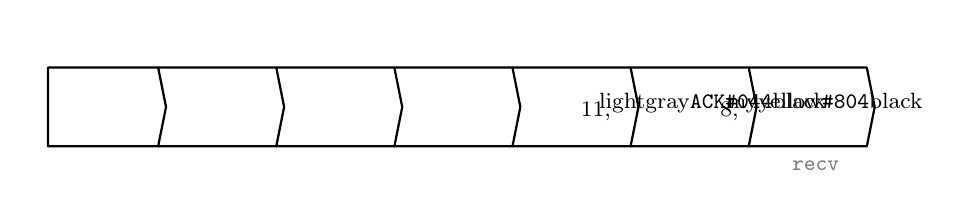
\begin{tikzpicture}
\draw[opacity=0] (-2.5,-1) rectangle (8.5,1);

\coordinate (mA) at (-1.5,0);
\coordinate (mB) at (0,0);
\coordinate (mC) at (1.5,0);
\coordinate (mD) at (3,0);
\coordinate (mE) at (4.5,0);
\coordinate (mF) at (6,0);
\coordinate (mG) at (7.5,0);

\pic at (mG) {queuenode={white}};
\pic at (mF) {queuenode={white}};
\pic at (mE) {queuenode={white}};
\pic at (mD) {queuenode={white}};
\pic at (mC) {queuenode={white}};
\pic at (mB) {queuenode={white}};
\pic at (mA) {queuenodetail={white}};

\node[smallgraytext] at (7.5,-0.75) {\texttt{recv}};

\node at (mF) {\footnotesize\hspace{1.5mm}11,\hspace{-1.5mm}\raisebox{1mm}{\bpacketid{lightgray}{\texttt{ACK}\\[-1.5mm]\texttt{\#044}}{black}}};
\node at (mG) {\footnotesize\hspace{1.5mm}8,\hspace{-1.5mm}\raisebox{1mm}{\bpacketid{myyellow}{\texttt{\#804}}{black}}};


\end{tikzpicture}
\end{figure}

\item \highlight{\textbf{send queue}} \\
\graytext{a min priority queue that stores packets waiting to be sent } \\[1mm]
\begin{figure}
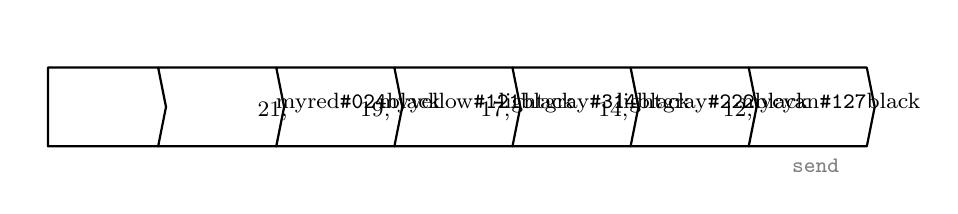
\begin{tikzpicture}
\draw[opacity=0] (-2.5,-1) rectangle (8.5,1);

\coordinate (mA) at (-1.5,0);
\coordinate (mB) at (0,0);
\coordinate (mC) at (1.5,0);
\coordinate (mD) at (3,0);
\coordinate (mE) at (4.5,0);
\coordinate (mF) at (6,0);
\coordinate (mG) at (7.5,0);

\pic at (mG) {queuenode={white}};
\pic at (mF) {queuenode={white}};
\pic at (mE) {queuenode={white}};
\pic at (mD) {queuenode={white}};
\pic at (mC) {queuenode={white}};
\pic at (mB) {queuenode={white}};
\pic at (mA) {queuenodetail={white}};

\node[smallgraytext] at (7.5,-0.75) {\texttt{send}};

\node at (mC) {\footnotesize\hspace{1.5mm}21,\hspace{-1.5mm}\raisebox{1mm}{\bpacketid{myred}{\texttt{\#024}}{black}}};
\node at (mD) {\footnotesize\hspace{1.5mm}19,\hspace{-1.5mm}\raisebox{1mm}{\bpacketid{myyellow}{\texttt{\#121}}{black}}};
\node at (mE) {\footnotesize\hspace{1.5mm}17,\hspace{-1.5mm}\raisebox{1mm}{\bpacketid{lightgray}{\texttt{\#314}}{black}}};
\node at (mF) {\footnotesize\hspace{1.5mm}14,\hspace{-1.5mm}\raisebox{1mm}{\bpacketid{lightgray}{\texttt{\#222}}{black}}};
\node at (mG) {\footnotesize\hspace{1.5mm}12,\hspace{-1.5mm}\raisebox{1mm}{\bpacketid{mycyan}{\texttt{\#127}}{black}}};

\end{tikzpicture}
\end{figure}
\end{itemize}
\end{frame}

\begin{frame}
\begin{itemize}
\item \highlight{\textbf{deadline queue}} \\
\graytext{a min priority queue that stores when each packet's acknowledgement is due; \\ the priority is the deadline for the acknowledgement }

\begin{figure}
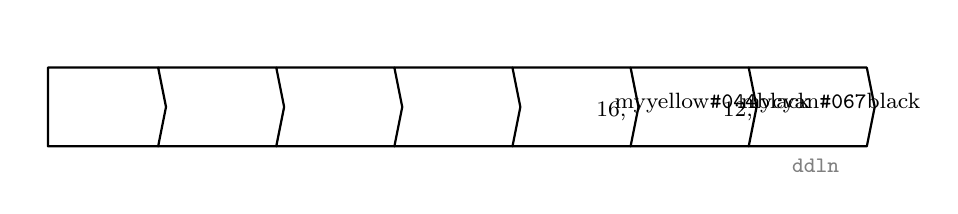
\begin{tikzpicture}
\draw[opacity=0] (-2.5,-1) rectangle (8.5,1);

\coordinate (mA) at (-1.5,0);
\coordinate (mB) at (0,0);
\coordinate (mC) at (1.5,0);
\coordinate (mD) at (3,0);
\coordinate (mE) at (4.5,0);
\coordinate (mF) at (6,0);
\coordinate (mG) at (7.5,0);

\pic at (mG) {queuenode={white}};
\pic at (mF) {queuenode={white}};
\pic at (mE) {queuenode={white}};
\pic at (mD) {queuenode={white}};
\pic at (mC) {queuenode={white}};
\pic at (mB) {queuenode={white}};
\pic at (mA) {queuenodetail={white}};

\node[smallgraytext] at (7.5,-0.75) {\texttt{ddln}};

\node at (mF) {\footnotesize\hspace{1.5mm}16,\hspace{-1.5mm}\raisebox{1mm}{\bpacketid{myyellow}{\texttt{\#044}}{black}}};
\node at (mG) {\footnotesize\hspace{1.5mm}12,\hspace{-1.5mm}\raisebox{1mm}{\bpacketid{mycyan}{\texttt{\#067}}{black}}};


\end{tikzpicture}
\end{figure}

\item \highlight{\textbf{acknowledgement table}} \\
\graytext{a dictionary mapping packet IDs to flags stating their acknowledgement status}\\

\begin{figure}
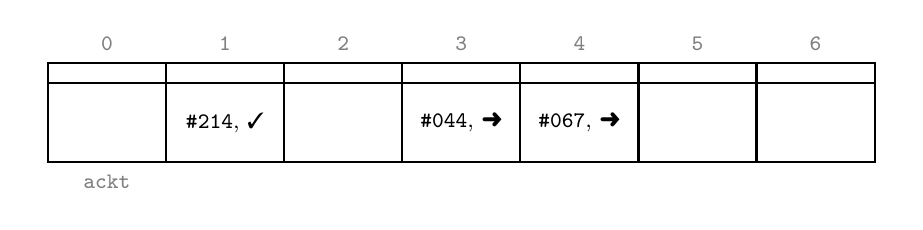
\begin{tikzpicture}
\draw[opacity=0] (-2.5,-1) rectangle (8.5,1);
\coordinate (mZ) at (-1.5,0);
\coordinate (mA) at (0,0);
\coordinate (mB) at (1.5,0);
\coordinate (mC) at (3,0);
\coordinate (mD) at (4.5,0);
\coordinate (mE) at (6,0);
\coordinate (mF) at (7.5,0);

\pic at (mZ) {dictnode={white}};
\pic at (mA) {dictnode={white}};
\pic at (mB) {dictnode={white}}; 
\pic at (mC) {dictnode={white}};
\pic at (mD) {dictnode={white}};
\pic at (mE) {dictnode={white}};
\pic at (mF) {dictnode={white}};

\node[smallgraytext] (l1) at (-1.5,1) {\texttt{0}};
\node[smallgraytext] (l2) at (0,1) {\texttt{1}};
\node[smallgraytext] (l3) at (1.5,1) {\texttt{2}};
\node[smallgraytext] (l4) at (3,1) {\texttt{3}};
\node[smallgraytext] (l5) at (4.5, 1) {\texttt{4}};
\node[smallgraytext] (l6) at (6,1) {\texttt{5}};
\node[smallgraytext] (l7) at (7.5,1) {\texttt{6}};

\node[smallgraytext] at (-1.5,-0.75) {\texttt{ackt}};

\node[draw opacity=0] at (mA) {\footnotesize \texttt{\#214},\hspace{1mm}\ding{51}};
\node[draw opacity=0] at (mC) {\footnotesize \texttt{\#044},\hspace{1mm}\ding{220}};
\node[draw opacity=0] at (mD) {\footnotesize \texttt{\#067},\hspace{1mm}\ding{220}};


\end{tikzpicture}
\end{figure}

\end{itemize}
\end{frame}


\begin{frame}
\vspace{2mm}
\begin{figure}
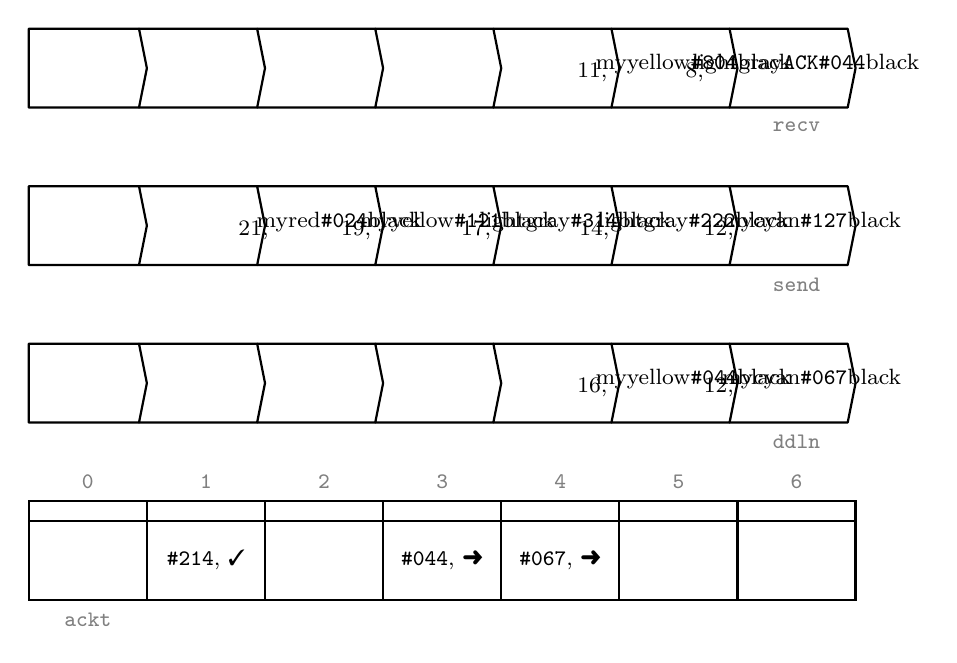
\begin{tikzpicture}

\begin{scope}

\coordinate (mA) at (-1.5,0);
\coordinate (mB) at (0,0);
\coordinate (mC) at (1.5,0);
\coordinate (mD) at (3,0);
\coordinate (mE) at (4.5,0);
\coordinate (mF) at (6,0);
\coordinate (mG) at (7.5,0);

\pic at (mG) {queuenode={white}};
\pic at (mF) {queuenode={white}};
\pic at (mE) {queuenode={white}};
\pic at (mD) {queuenode={white}};
\pic at (mC) {queuenode={white}};
\pic at (mB) {queuenode={white}};
\pic at (mA) {queuenodetail={white}};


\node[smallgraytext] at (7.5,-0.75) {\texttt{recv}};

\node (p1) at (mG) {\footnotesize\hspace{1.5mm}8,\hspace{-1.5mm}\raisebox{1mm}{\bpacketid{lightgray}{\texttt{ACK}\\[-1.5mm]\texttt{\#044}}{black}}};
\node (p2) at (mF) {\footnotesize\hspace{1.5mm}11,\hspace{-1.5mm}\raisebox{1mm}{\bpacketid{myyellow}{\texttt{\#804}}{black}}};


\end{scope}

\begin{scope}[yshift=-2cm]

\coordinate (mA) at (-1.5,0);
\coordinate (mB) at (0,0);
\coordinate (mC) at (1.5,0);
\coordinate (mD) at (3,0);
\coordinate (mE) at (4.5,0);
\coordinate (mF) at (6,0);
\coordinate (mG) at (7.5,0);

\pic at (mG) {queuenode={white}};
\pic at (mF) {queuenode={white}};
\pic at (mE) {queuenode={white}};
\pic at (mD) {queuenode={white}};
\pic at (mC) {queuenode={white}};
\pic at (mB) {queuenode={white}};
\pic at (mA) {queuenodetail={white}};

\node[smallgraytext] at (7.5,-0.75) {\texttt{send}};

\node (p1) at (mC) {\footnotesize\hspace{1.5mm}21,\hspace{-1.5mm}\raisebox{1mm}{\bpacketid{myred}{\texttt{\#024}}{black}}};
\node (p2) at (mD) {\footnotesize\hspace{1.5mm}19,\hspace{-1.5mm}\raisebox{1mm}{\bpacketid{myyellow}{\texttt{\#121}}{black}}};
\node (p3) at (mE) {\footnotesize\hspace{1.5mm}17,\hspace{-1.5mm}\raisebox{1mm}{\bpacketid{lightgray}{\texttt{\#314}}{black}}};
\node (p4) at (mF) {\footnotesize\hspace{1.5mm}14,\hspace{-1.5mm}\raisebox{1mm}{\bpacketid{lightgray}{\texttt{\#222}}{black}}};
\node (p5) at (mG) {\footnotesize\hspace{1.5mm}12,\hspace{-1.5mm}\raisebox{1mm}{\bpacketid{mycyan}{\texttt{\#127}}{black}}};


\end{scope}

\begin{scope}[yshift=-4cm]

\coordinate (mA) at (-1.5,0);
\coordinate (mB) at (0,0);
\coordinate (mC) at (1.5,0);
\coordinate (mD) at (3,0);
\coordinate (mE) at (4.5,0);
\coordinate (mF) at (6,0);
\coordinate (mG) at (7.5,0);

\pic at (mG) {queuenode={white}};
\pic at (mF) {queuenode={white}};
\pic at (mE) {queuenode={white}};
\pic at (mD) {queuenode={white}};
\pic at (mC) {queuenode={white}};
\pic at (mB) {queuenode={white}};
\pic at (mA) {queuenodetail={white}};

\node[smallgraytext] at (7.5,-0.75) {\texttt{ddln}};

\node at (mF) {\footnotesize\hspace{1.5mm}16,\hspace{-1.5mm}\raisebox{1mm}{\bpacketid{myyellow}{\texttt{\#044}}{black}}};
\node at (mG) {\footnotesize\hspace{1.5mm}12,\hspace{-1.5mm}\raisebox{1mm}{\bpacketid{mycyan}{\texttt{\#067}}{black}}};

\end{scope}

\begin{scope}[yshift=-6.25cm]

\coordinate (mZ) at (-1.5,0);
\coordinate (mA) at (0,0);
\coordinate (mB) at (1.5,0);
\coordinate (mC) at (3,0);
\coordinate (mD) at (4.5,0);
\coordinate (mE) at (6,0);
\coordinate (mF) at (7.5,0);

\pic at (mZ) {dictnode={white}};
\pic at (mA) {dictnode={white}};
\pic at (mB) {dictnode={white}}; 
\pic at (mC) {dictnode={white}};
\pic at (mD) {dictnode={white}};
\pic at (mE) {dictnode={white}};
\pic at (mF) {dictnode={white}};

\node[smallgraytext] (l1) at (-1.5,1) {\texttt{0}};
\node[smallgraytext] (l2) at (0,1) {\texttt{1}};
\node[smallgraytext] (l3) at (1.5,1) {\texttt{2}};
\node[smallgraytext] (l4) at (3,1) {\texttt{3}};
\node[smallgraytext] (l5) at (4.5, 1) {\texttt{4}};
\node[smallgraytext] (l6) at (6,1) {\texttt{5}};
\node[smallgraytext] (l7) at (7.5,1) {\texttt{6}};

\node[smallgraytext] at (-1.5,-0.75) {\texttt{ackt}};

\node[draw opacity=0] at (mA) {\footnotesize \texttt{\#214},\hspace{1mm}\ding{51}};
\node[draw opacity=0] at (mC) {\footnotesize \texttt{\#044},\hspace{1mm}\ding{220}};
\node[draw opacity=0] at (mD) {\footnotesize \texttt{\#067},\hspace{1mm}\ding{220}};


\end{scope}

\end{tikzpicture}
\end{figure}
\vspace{-6mm}
\begin{center}
\graytext{the tower's data at the start of time-step $t = 12$ \\ \;}
\end{center}
\end{frame}

\begin{frame}
\vspace{2mm}
\begin{figure}
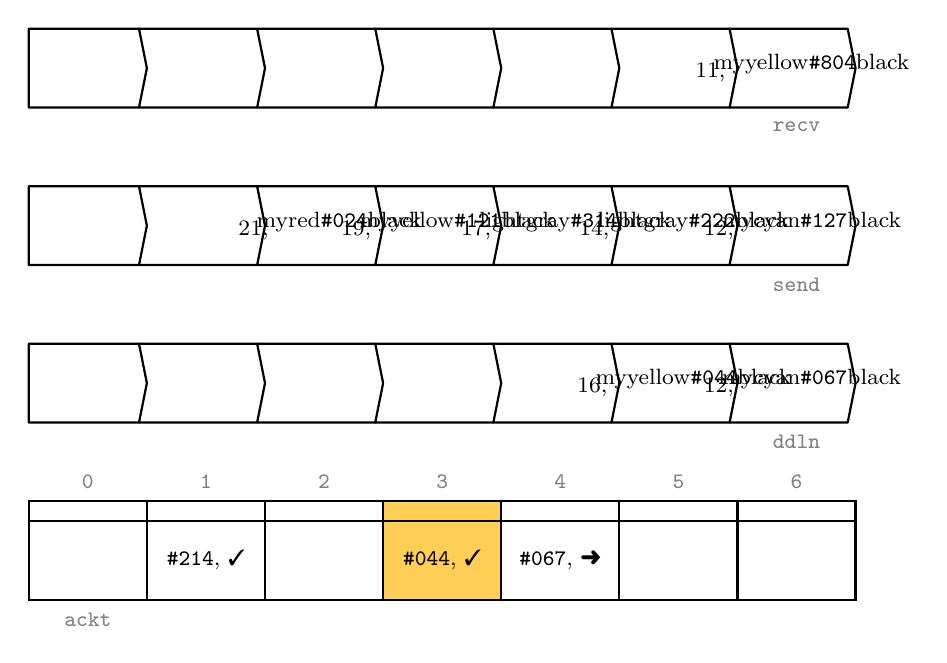
\begin{tikzpicture}

\begin{scope}

\coordinate (mA) at (-1.5,0);
\coordinate (mB) at (0,0);
\coordinate (mC) at (1.5,0);
\coordinate (mD) at (3,0);
\coordinate (mE) at (4.5,0);
\coordinate (mF) at (6,0);
\coordinate (mG) at (7.5,0);

\pic at (mG) {queuenode={white}};
\pic at (mF) {queuenode={white}};
\pic at (mE) {queuenode={white}};
\pic at (mD) {queuenode={white}};
\pic at (mC) {queuenode={white}};
\pic at (mB) {queuenode={white}};
\pic at (mA) {queuenodetail={white}};


\node[smallgraytext] at (7.5,-0.75) {\texttt{recv}};

\node (p2) at (mG) {\footnotesize\hspace{1.5mm}11,\hspace{-1.5mm}\raisebox{1mm}{\bpacketid{myyellow}{\texttt{\#804}}{black}}};

\end{scope}

\begin{scope}[yshift=-2cm]

\coordinate (mA) at (-1.5,0);
\coordinate (mB) at (0,0);
\coordinate (mC) at (1.5,0);
\coordinate (mD) at (3,0);
\coordinate (mE) at (4.5,0);
\coordinate (mF) at (6,0);
\coordinate (mG) at (7.5,0);

\pic at (mG) {queuenode={white}};
\pic at (mF) {queuenode={white}};
\pic at (mE) {queuenode={white}};
\pic at (mD) {queuenode={white}};
\pic at (mC) {queuenode={white}};
\pic at (mB) {queuenode={white}};
\pic at (mA) {queuenodetail={white}};


\node[smallgraytext] at (7.5,-0.75) {\texttt{send}};

\node (p1) at (mC) {\footnotesize\hspace{1.5mm}21,\hspace{-1.5mm}\raisebox{1mm}{\bpacketid{myred}{\texttt{\#024}}{black}}};
\node (p2) at (mD) {\footnotesize\hspace{1.5mm}19,\hspace{-1.5mm}\raisebox{1mm}{\bpacketid{myyellow}{\texttt{\#121}}{black}}};
\node (p3) at (mE) {\footnotesize\hspace{1.5mm}17,\hspace{-1.5mm}\raisebox{1mm}{\bpacketid{lightgray}{\texttt{\#314}}{black}}};
\node (p4) at (mF) {\footnotesize\hspace{1.5mm}14,\hspace{-1.5mm}\raisebox{1mm}{\bpacketid{lightgray}{\texttt{\#222}}{black}}};
\node (p5) at (mG) {\footnotesize\hspace{1.5mm}12,\hspace{-1.5mm}\raisebox{1mm}{\bpacketid{mycyan}{\texttt{\#127}}{black}}};


\end{scope}

\begin{scope}[yshift=-4cm]

\coordinate (mA) at (-1.5,0);
\coordinate (mB) at (0,0);
\coordinate (mC) at (1.5,0);
\coordinate (mD) at (3,0);
\coordinate (mE) at (4.5,0);
\coordinate (mF) at (6,0);
\coordinate (mG) at (7.5,0);

\pic at (mG) {queuenode={white}};
\pic at (mF) {queuenode={white}};
\pic at (mE) {queuenode={white}};
\pic at (mD) {queuenode={white}};
\pic at (mC) {queuenode={white}};
\pic at (mB) {queuenode={white}};
\pic at (mA) {queuenodetail={white}};


\node[smallgraytext] at (7.5,-0.75) {\texttt{ddln}};

\node at (mF) {\footnotesize\hspace{1.5mm}16,\hspace{-1.5mm}\raisebox{1mm}{\bpacketid{myyellow}{\texttt{\#044}}{black}}};
\node at (mG) {\footnotesize\hspace{1.5mm}12,\hspace{-1.5mm}\raisebox{1mm}{\bpacketid{mycyan}{\texttt{\#067}}{black}}};

\end{scope}

\begin{scope}[yshift=-6.25cm]

\coordinate (mZ) at (-1.5,0);
\coordinate (mA) at (0,0);
\coordinate (mB) at (1.5,0);
\coordinate (mC) at (3,0);
\coordinate (mD) at (4.5,0);
\coordinate (mE) at (6,0);
\coordinate (mF) at (7.5,0);

\pic at (mZ) {dictnode={white}};
\pic at (mA) {dictnode={white}};
\pic at (mB) {dictnode={white}}; 
\pic at (mC) {dictnode={myyellow}};
\pic at (mD) {dictnode={white}};
\pic at (mE) {dictnode={white}};
\pic at (mF) {dictnode={white}};

\node[smallgraytext] (l1) at (-1.5,1) {\texttt{0}};
\node[smallgraytext] (l2) at (0,1) {\texttt{1}};
\node[smallgraytext] (l3) at (1.5,1) {\texttt{2}};
\node[smallgraytext] (l4) at (3,1) {\texttt{3}};
\node[smallgraytext] (l5) at (4.5, 1) {\texttt{4}};
\node[smallgraytext] (l6) at (6,1) {\texttt{5}};
\node[smallgraytext] (l7) at (7.5,1) {\texttt{6}};

\node[smallgraytext] at (-1.5,-0.75) {\texttt{ackt}};

\node[draw opacity=0] at (mA) {\footnotesize \texttt{\#214},\hspace{1mm}\ding{51}};
\node[draw opacity=0] at (mC) {\footnotesize \texttt{\#044},\hspace{1mm}\ding{51}};
\node[draw opacity=0] at (mD) {\footnotesize \texttt{\#067},\hspace{1mm}\ding{220}};


\end{scope}

\end{tikzpicture}
\end{figure}
\vspace{-6mm}
\begin{center}
\graytext{\texttt{recv} is processed;\\\texttt{ACK \#044} is updated in \texttt{ackt}}
\end{center}
\end{frame}

\begin{frame}
\vspace{2mm}
\begin{figure}
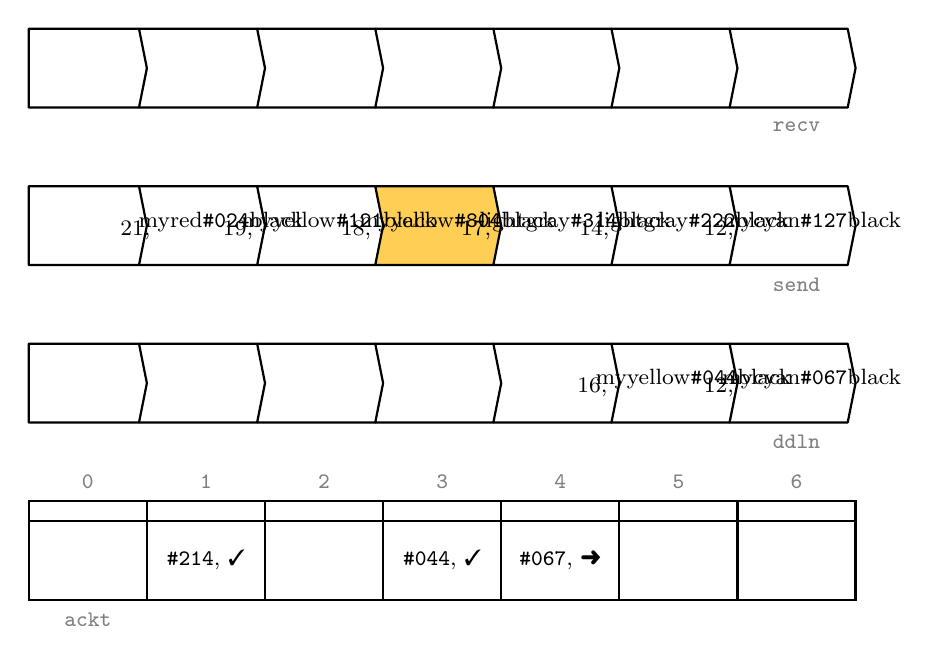
\begin{tikzpicture}

\begin{scope}

\coordinate (mA) at (-1.5,0);
\coordinate (mB) at (0,0);
\coordinate (mC) at (1.5,0);
\coordinate (mD) at (3,0);
\coordinate (mE) at (4.5,0);
\coordinate (mF) at (6,0);
\coordinate (mG) at (7.5,0);

\pic at (mG) {queuenode={white}};
\pic at (mF) {queuenode={white}};
\pic at (mE) {queuenode={white}};
\pic at (mD) {queuenode={white}};
\pic at (mC) {queuenode={white}};
\pic at (mB) {queuenode={white}};
\pic at (mA) {queuenodetail={white}};


\node[smallgraytext] at (7.5,-0.75) {\texttt{recv}};

\end{scope}

\begin{scope}[yshift=-2cm]

\coordinate (mA) at (-1.5,0);
\coordinate (mB) at (0,0);
\coordinate (mC) at (1.5,0);
\coordinate (mD) at (3,0);
\coordinate (mE) at (4.5,0);
\coordinate (mF) at (6,0);
\coordinate (mG) at (7.5,0);

\pic at (mG) {queuenode={white}};
\pic at (mF) {queuenode={white}};
\pic at (mE) {queuenode={white}};
\pic at (mD) {queuenode={myyellow}};
\pic at (mC) {queuenode={white}};
\pic at (mB) {queuenode={white}};
\pic at (mA) {queuenodetail={white}};


\node[smallgraytext] at (7.5,-0.75) {\texttt{send}};

\node (p0) at (mD) {\footnotesize\hspace{1.5mm}18,\hspace{-1.5mm}\raisebox{1mm}{\bpacketid{myyellow}{\texttt{\#804}}{black}}};
\node (p1) at (mB) {\footnotesize\hspace{1.5mm}21,\hspace{-1.5mm}\raisebox{1mm}{\bpacketid{myred}{\texttt{\#024}}{black}}};
\node (p2) at (mC) {\footnotesize\hspace{1.5mm}19,\hspace{-1.5mm}\raisebox{1mm}{\bpacketid{myyellow}{\texttt{\#121}}{black}}};
\node (p3) at (mE) {\footnotesize\hspace{1.5mm}17,\hspace{-1.5mm}\raisebox{1mm}{\bpacketid{lightgray}{\texttt{\#314}}{black}}};
\node (p4) at (mF) {\footnotesize\hspace{1.5mm}14,\hspace{-1.5mm}\raisebox{1mm}{\bpacketid{lightgray}{\texttt{\#222}}{black}}};
\node (p5) at (mG) {\footnotesize\hspace{1.5mm}12,\hspace{-1.5mm}\raisebox{1mm}{\bpacketid{mycyan}{\texttt{\#127}}{black}}};


\end{scope}

\begin{scope}[yshift=-4cm]

\coordinate (mA) at (-1.5,0);
\coordinate (mB) at (0,0);
\coordinate (mC) at (1.5,0);
\coordinate (mD) at (3,0);
\coordinate (mE) at (4.5,0);
\coordinate (mF) at (6,0);
\coordinate (mG) at (7.5,0);

\pic at (mG) {queuenode={white}};
\pic at (mF) {queuenode={white}};
\pic at (mE) {queuenode={white}};
\pic at (mD) {queuenode={white}};
\pic at (mC) {queuenode={white}};
\pic at (mB) {queuenode={white}};
\pic at (mA) {queuenodetail={white}};

\node[smallgraytext] at (7.5,-0.75) {\texttt{ddln}};

\node at (mF) {\footnotesize\hspace{1.5mm}16,\hspace{-1.5mm}\raisebox{1mm}{\bpacketid{myyellow}{\texttt{\#044}}{black}}};
\node at (mG) {\footnotesize\hspace{1.5mm}12,\hspace{-1.5mm}\raisebox{1mm}{\bpacketid{mycyan}{\texttt{\#067}}{black}}};


\end{scope}

\begin{scope}[yshift=-6.25cm]

\coordinate (mZ) at (-1.5,0);
\coordinate (mA) at (0,0);
\coordinate (mB) at (1.5,0);
\coordinate (mC) at (3,0);
\coordinate (mD) at (4.5,0);
\coordinate (mE) at (6,0);
\coordinate (mF) at (7.5,0);

\pic at (mZ) {dictnode={white}};
\pic at (mA) {dictnode={white}};
\pic at (mB) {dictnode={white}}; 
\pic at (mC) {dictnode={white}};
\pic at (mD) {dictnode={white}};
\pic at (mE) {dictnode={white}};
\pic at (mF) {dictnode={white}};

\node[smallgraytext] (l1) at (-1.5,1) {\texttt{0}};
\node[smallgraytext] (l2) at (0,1) {\texttt{1}};
\node[smallgraytext] (l3) at (1.5,1) {\texttt{2}};
\node[smallgraytext] (l4) at (3,1) {\texttt{3}};
\node[smallgraytext] (l5) at (4.5, 1) {\texttt{4}};
\node[smallgraytext] (l6) at (6,1) {\texttt{5}};
\node[smallgraytext] (l7) at (7.5,1) {\texttt{6}};
\node[smallgraytext] at (-1.5,-0.75) {\texttt{ackt}};

\node[draw opacity=0] at (mA) {\footnotesize \texttt{\#214},\hspace{1mm}\ding{51}};
\node[draw opacity=0] at (mC) {\footnotesize \texttt{\#044},\hspace{1mm}\ding{51}};
\node[draw opacity=0] at (mD) {\footnotesize \texttt{\#067},\hspace{1mm}\ding{220}};


\end{scope}

\end{tikzpicture}
\end{figure}
\vspace{-6mm}
\begin{center}
\graytext{\texttt{recv} is processed;\\ \texttt{\#804} is assigned a priority of 18 and added to \texttt{send}}
\end{center}
\end{frame}

\begin{frame}
\vspace{2mm}
\begin{figure}
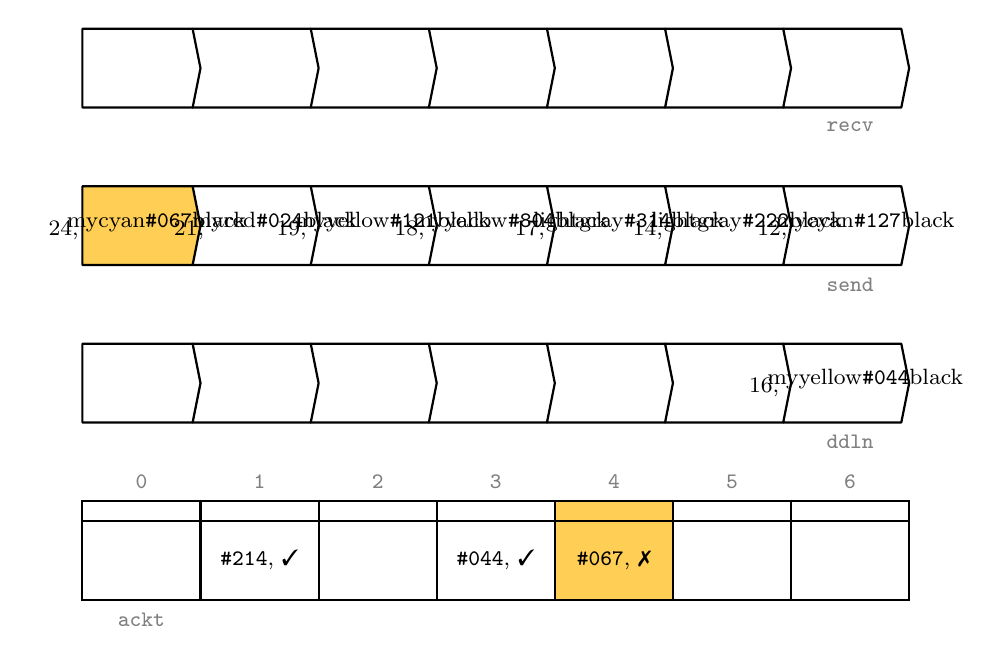
\begin{tikzpicture}

\begin{scope}

\coordinate (mA) at (-1.5,0);
\coordinate (mB) at (0,0);
\coordinate (mC) at (1.5,0);
\coordinate (mD) at (3,0);
\coordinate (mE) at (4.5,0);
\coordinate (mF) at (6,0);
\coordinate (mG) at (7.5,0);

\pic at (mG) {queuenode={white}};
\pic at (mF) {queuenode={white}};
\pic at (mE) {queuenode={white}};
\pic at (mD) {queuenode={white}};
\pic at (mC) {queuenode={white}};
\pic at (mB) {queuenode={white}};
\pic at (mA) {queuenodetail={white}};


\node[smallgraytext] at (7.5,-0.75) {\texttt{recv}};

\end{scope}

\begin{scope}[yshift=-2cm]

\coordinate (mA) at (-1.5,0);
\coordinate (mB) at (0,0);
\coordinate (mC) at (1.5,0);
\coordinate (mD) at (3,0);
\coordinate (mE) at (4.5,0);
\coordinate (mF) at (6,0);
\coordinate (mG) at (7.5,0);

\pic at (mG) {queuenode={white}};
\pic at (mF) {queuenode={white}};
\pic at (mE) {queuenode={white}};
\pic at (mD) {queuenode={white}};
\pic at (mC) {queuenode={white}};
\pic at (mB) {queuenode={white}};
\pic at (mA) {queuenodetail={myyellow}};


\node[smallgraytext] at (7.5,-0.75) {\texttt{send}};

\node (pm1) at (mA) {\footnotesize\hspace{1.5mm}24,\hspace{-1.5mm}\raisebox{1mm}{\bpacketid{mycyan}{\texttt{\#067}}{black}}};
\node (p0) at (mD) {\footnotesize\hspace{1.5mm}18,\hspace{-1.5mm}\raisebox{1mm}{\bpacketid{myyellow}{\texttt{\#804}}{black}}};
\node (p1) at (mB) {\footnotesize\hspace{1.5mm}21,\hspace{-1.5mm}\raisebox{1mm}{\bpacketid{myred}{\texttt{\#024}}{black}}};
\node (p2) at (mC) {\footnotesize\hspace{1.5mm}19,\hspace{-1.5mm}\raisebox{1mm}{\bpacketid{myyellow}{\texttt{\#121}}{black}}};
\node (p3) at (mE) {\footnotesize\hspace{1.5mm}17,\hspace{-1.5mm}\raisebox{1mm}{\bpacketid{lightgray}{\texttt{\#314}}{black}}};
\node (p4) at (mF) {\footnotesize\hspace{1.5mm}14,\hspace{-1.5mm}\raisebox{1mm}{\bpacketid{lightgray}{\texttt{\#222}}{black}}};
\node (p5) at (mG) {\footnotesize\hspace{1.5mm}12,\hspace{-1.5mm}\raisebox{1mm}{\bpacketid{mycyan}{\texttt{\#127}}{black}}};


\end{scope}

\begin{scope}[yshift=-4cm]

\coordinate (mA) at (-1.5,0);
\coordinate (mB) at (0,0);
\coordinate (mC) at (1.5,0);
\coordinate (mD) at (3,0);
\coordinate (mE) at (4.5,0);
\coordinate (mF) at (6,0);
\coordinate (mG) at (7.5,0);

\pic at (mG) {queuenode={white}};
\pic at (mF) {queuenode={white}};
\pic at (mE) {queuenode={white}};
\pic at (mD) {queuenode={white}};
\pic at (mC) {queuenode={white}};
\pic at (mB) {queuenode={white}};
\pic at (mA) {queuenodetail={white}};

\node[smallgraytext] at (7.5,-0.75) {\texttt{ddln}};

\node at (mG) {\footnotesize\hspace{1.5mm}16,\hspace{-1.5mm}\raisebox{1mm}{\bpacketid{myyellow}{\texttt{\#044}}{black}}};


\end{scope}

\begin{scope}[yshift=-6.25cm]

\coordinate (mZ) at (-1.5,0);
\coordinate (mA) at (0,0);
\coordinate (mB) at (1.5,0);
\coordinate (mC) at (3,0);
\coordinate (mD) at (4.5,0);
\coordinate (mE) at (6,0);
\coordinate (mF) at (7.5,0);

\pic at (mZ) {dictnode={white}};
\pic at (mA) {dictnode={white}};
\pic at (mB) {dictnode={white}}; 
\pic at (mC) {dictnode={white}};
\pic at (mD) {dictnode={myyellow}};
\pic at (mE) {dictnode={white}};
\pic at (mF) {dictnode={white}};

\node[smallgraytext] (l1) at (-1.5,1) {\texttt{0}};
\node[smallgraytext] (l2) at (0,1) {\texttt{1}};
\node[smallgraytext] (l3) at (1.5,1) {\texttt{2}};
\node[smallgraytext] (l4) at (3,1) {\texttt{3}};
\node[smallgraytext] (l5) at (4.5, 1) {\texttt{4}};
\node[smallgraytext] (l6) at (6,1) {\texttt{5}};
\node[smallgraytext] (l7) at (7.5,1) {\texttt{6}};

\node[smallgraytext] at (-1.5,-0.75) {\texttt{ackt}};

\node[draw opacity=0] at (mA) {\footnotesize \texttt{\#214},\hspace{1mm}\ding{51}};
\node[draw opacity=0] at (mC) {\footnotesize \texttt{\#044},\hspace{1mm}\ding{51}};
\node[draw opacity=0] at (mD) {\footnotesize \texttt{\#067},\hspace{1mm}\ding{55}};

\end{scope}

\end{tikzpicture}
\end{figure}
\vspace{-6mm}
\begin{center}
\graytext{\texttt{ddln} is processed;\\ \texttt{\#067} is updated in \texttt{ackt}, assigned a priority of \texttt{24}, and then added to \texttt{send}}
\end{center}
\end{frame}

\begin{frame}
\vspace{2mm}
\begin{figure}
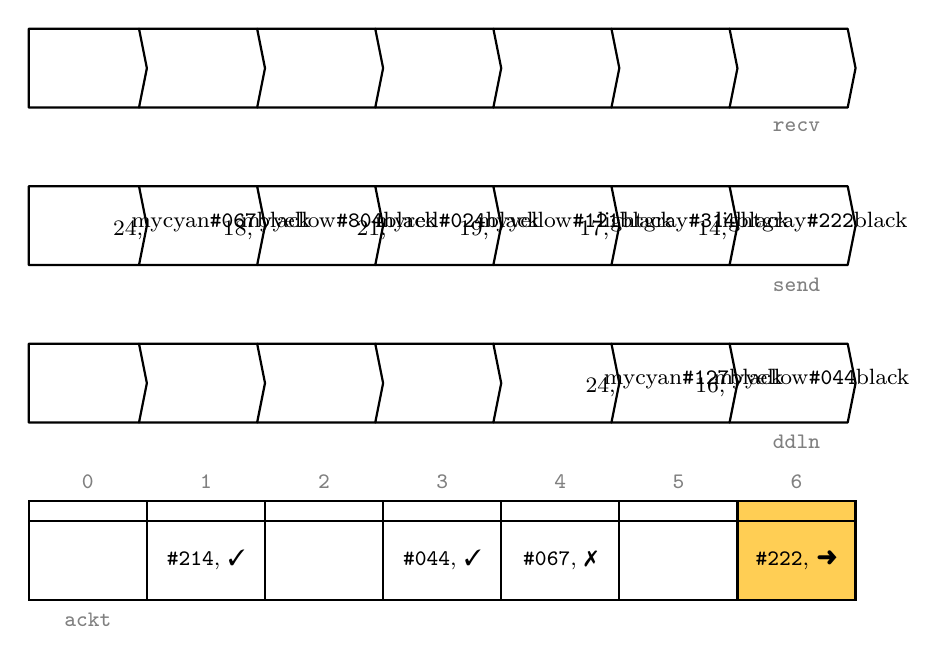
\begin{tikzpicture}

\begin{scope}

\coordinate (mA) at (-1.5,0);
\coordinate (mB) at (0,0);
\coordinate (mC) at (1.5,0);
\coordinate (mD) at (3,0);
\coordinate (mE) at (4.5,0);
\coordinate (mF) at (6,0);
\coordinate (mG) at (7.5,0);

\pic at (mG) {queuenode={white}};
\pic at (mF) {queuenode={white}};
\pic at (mE) {queuenode={white}};
\pic at (mD) {queuenode={white}};
\pic at (mC) {queuenode={white}};
\pic at (mB) {queuenode={white}};
\pic at (mA) {queuenodetail={white}};


\node[smallgraytext] at (7.5,-0.75) {\texttt{recv}};

\end{scope}

\begin{scope}[yshift=-2cm]

\coordinate (mA) at (-1.5,0);
\coordinate (mB) at (0,0);
\coordinate (mC) at (1.5,0);
\coordinate (mD) at (3,0);
\coordinate (mE) at (4.5,0);
\coordinate (mF) at (6,0);
\coordinate (mG) at (7.5,0);

\pic at (mG) {queuenode={white}};
\pic at (mF) {queuenode={white}};
\pic at (mE) {queuenode={white}};
\pic at (mD) {queuenode={white}};
\pic at (mC) {queuenode={white}};
\pic at (mB) {queuenode={white}};
\pic at (mA) {queuenodetail={white}};


\node[smallgraytext] at (7.5,-0.75) {\texttt{send}};

\node (pm1) at (mB) {\footnotesize\hspace{1.5mm}24,\hspace{-1.5mm}\raisebox{1mm}{\bpacketid{mycyan}{\texttt{\#067}}{black}}};
\node (p0) at (mC) {\footnotesize\hspace{1.5mm}18,\hspace{-1.5mm}\raisebox{1mm}{\bpacketid{myyellow}{\texttt{\#804}}{black}}};
\node (p1) at (mD) {\footnotesize\hspace{1.5mm}21,\hspace{-1.5mm}\raisebox{1mm}{\bpacketid{myred}{\texttt{\#024}}{black}}};
\node (p2) at (mE) {\footnotesize\hspace{1.5mm}19,\hspace{-1.5mm}\raisebox{1mm}{\bpacketid{myyellow}{\texttt{\#121}}{black}}};
\node (p3) at (mF) {\footnotesize\hspace{1.5mm}17,\hspace{-1.5mm}\raisebox{1mm}{\bpacketid{lightgray}{\texttt{\#314}}{black}}};
\node (p4) at (mG) {\footnotesize\hspace{1.5mm}14,\hspace{-1.5mm}\raisebox{1mm}{\bpacketid{lightgray}{\texttt{\#222}}{black}}};


\end{scope}

\begin{scope}[yshift=-4cm]

\coordinate (mA) at (-1.5,0);
\coordinate (mB) at (0,0);
\coordinate (mC) at (1.5,0);
\coordinate (mD) at (3,0);
\coordinate (mE) at (4.5,0);
\coordinate (mF) at (6,0);
\coordinate (mG) at (7.5,0);

\pic at (mG) {queuenode={white}};
\pic at (mF) {queuenode={white}};
\pic at (mE) {queuenode={white}};
\pic at (mD) {queuenode={white}};
\pic at (mC) {queuenode={white}};
\pic at (mB) {queuenode={white}};
\pic at (mA) {queuenodetail={white}};


\node[smallgraytext] at (7.5,-0.75) {\texttt{ddln}};

\node at (mG) {\footnotesize\hspace{1.5mm}16,\hspace{-1.5mm}\raisebox{1mm}{\bpacketid{myyellow}{\texttt{\#044}}{black}}};
\node at (mF) {\footnotesize\hspace{1.5mm}24,\hspace{-1.5mm}\raisebox{1mm}{\bpacketid{mycyan}{\texttt{\#127}}{black}}};


\end{scope}

\begin{scope}[yshift=-6.25cm]

\coordinate (mZ) at (-1.5,0);
\coordinate (mA) at (0,0);
\coordinate (mB) at (1.5,0);
\coordinate (mC) at (3,0);
\coordinate (mD) at (4.5,0);
\coordinate (mE) at (6,0);
\coordinate (mF) at (7.5,0);

\pic at (mZ) {dictnode={white}};
\pic at (mA) {dictnode={white}};
\pic at (mB) {dictnode={white}}; 
\pic at (mC) {dictnode={white}};
\pic at (mD) {dictnode={white}};
\pic at (mE) {dictnode={white}};
\pic at (mF) {dictnode={myyellow}};

\node[smallgraytext] (l1) at (-1.5,1) {\texttt{0}};
\node[smallgraytext] (l2) at (0,1) {\texttt{1}};
\node[smallgraytext] (l3) at (1.5,1) {\texttt{2}};
\node[smallgraytext] (l4) at (3,1) {\texttt{3}};
\node[smallgraytext] (l5) at (4.5, 1) {\texttt{4}};
\node[smallgraytext] (l6) at (6,1) {\texttt{5}};
\node[smallgraytext] (l7) at (7.5,1) {\texttt{6}};

\node[smallgraytext] at (-1.5,-0.75) {\texttt{ackt}};

\node[draw opacity=0] at (mA) {\footnotesize \texttt{\#214},\hspace{1mm}\ding{51}};
\node[draw opacity=0] at (mC) {\footnotesize \texttt{\#044},\hspace{1mm}\ding{51}};
\node[draw opacity=0] at (mD) {\footnotesize \texttt{\#067},\hspace{1mm}\ding{55}};
\node[draw opacity=0] at (mF) {\footnotesize \texttt{\#222},\hspace{1mm}\ding{220}};

\end{scope}

\end{tikzpicture}
\end{figure}
\vspace{-6mm}
\begin{center}
\graytext{\texttt{send} is processed;\\ \texttt{\#222} is sent, updated in \texttt{ackt}, and added to \texttt{ddln} with a value of \texttt{24}}
\end{center}
\end{frame}


\end{document}